\documentclass[12pt]{article}
\usepackage{natbib}
\usepackage[french]{babel}
\usepackage{url}
\usepackage[utf8x]{inputenc}
\usepackage{graphicx}
\graphicspath{{images/}}
\usepackage{parskip}
\usepackage{fancyhdr}
\usepackage{vmargin}
\usepackage{xcolor}
\usepackage{bbm}
\usepackage{amsmath,amssymb}
\usepackage{amsthm}
\usepackage{dsfont}
\usepackage{stmaryrd}
\usepackage{systeme}
\usepackage{enumitem}
\usepackage{xcolor}
\usepackage{pifont}
\usepackage[cache=false]{minted}
\definecolor{LightGray}{gray}{0.95}


\title{Polynômes de Permutations}
\author{PIARD A. - JACQUET R. - CARVAILLO T.}
\date{\today}

\makeatletter
\let\thetitle\@title
\let\theauthor\@author
\let\thedate\@date
\makeatother

\pagestyle{fancy}
\fancyhf{}
\rhead{\theauthor}
\lhead{\thetitle}
\cfoot{\thepage}
\def\dotfill#1{\cleaders\hbox to #1{.}\hfill}
\newcommand\dotline[2][.5em]{\leavevmode\hbox to #2{\dotfill{#1}\hfil}}

\newcommand{\M}{\mathbbm{M}}
\newcommand{\N}{\mathbbm{N}}
\newcommand{\Z}{\mathbbm{Z}}
\newcommand{\Q}{\mathbbm{Q}}
\newcommand{\R}{\mathbbm{R}}
\newcommand{\C}{\mathbbm{C}}
\newcommand{\G}{\mathbbm{G}}
\newcommand{\K}{\mathbbm{K}}
\newcommand{\F}{\mathbbm{F}}
\newcommand{\Fq}{\mathbbm{F}_q}

%définition commande présentation fonction
\newcommand{\fonction}[5]{
\begin{displaymath}
\begin{array}{l|rcl}
\displaystyle
#1 : & #2 & \longrightarrow & #3 \\
    & #4 & \longmapsto & #5
\end{array}
\end{displaymath}
}

%fin définition


% de jolies accolades
\newcommand{\accolade}[2]{
\begin{displaymath}
%#1 = \left\{
    \begin{array}{ll}
       #1 %& \mbox{si }
       #2 %& \mbox{sinon.}
    \end{array}
\right.
\end{displaymath}
}
% de jolies accolades




\newtheorem{theorem}{Théorème}
\newtheorem{corollaire}{Corollaire}
\newtheorem{lemma}{Lemme}
\newtheorem{prop}{Proposition}
\theoremstyle{definition}
\newtheorem{definition}{Définition}
\newtheorem{example}{Exemple}
\newtheorem*{examples}{Exemples}
\newtheorem{exo}{Exercice}	
\newtheorem{coro}{Corollaire}	
\newtheorem{rem}{Remarque}
\newtheorem{crit}{Critère}
\newtheorem{bg}{A l'attention des bg, question}

\begin{document}

%%%%%%%%%%%%%%%%%%%%%%%%%%%%%%%%%%%%%%%%%%%%%%%%%%%%%%%%%%%%%%%%%%%%%%%%%%%%%%%%%%%%%%%%%

\begin{titlepage}
	\centering
    \vspace*{0.5 cm}
    \textsc{\LARGE Projet de Recherche . 2020-2021}\\[1.0 cm]
    \dotline[15pt]{15cm}\\
	
\includegraphics[scale = 2.2]{logo.png}
	\dotline[15pt]{15cm}\\
	\vspace{1.5cm}
	\textsc{\Large Faculté des Sciences et Techniques}\\
	\textsc{\large Master 1 - Maths. CRYPTIS}\\[1.0 cm]
	\rule{\linewidth}{0.2 mm} \\[0.4 cm]
	{ \huge \bfseries \color{blue} \thetitle}\\
	\rule{\linewidth}{0.2 mm} \\[1.5 cm]
	
	\begin{minipage}{0.4\textwidth}
		\begin{flushleft} \large
			\emph{A l'attention de :}\\
			M. NECER\\
			\phantom{a}\\
			\phantom{a}\\
		\end{flushleft}
	\end{minipage}
	\begin{minipage}{0.5\textwidth}
    	\begin{flushright} \large
		\emph{Rédigé par :}\\
		PIARD A.\\
		JACQUET R.\\
		CARVAILLO T.\\
		\end{flushright}
	\end{minipage}\\[2 cm]
\end{titlepage}

%%%%%%%%%%%%%%%%%%%%%%%%%%%%%%%%%%%%%%%%%%%%%%%%%%%%%%%%%%%%%%%%%%%%%%%%%%%%%%%%%%%%%%%%%

\tableofcontents
\pagebreak
\section*{\Huge Notation}

\vspace{3cm}
\begin{tabular}{p{4cm}p{15cm}}
$\mathbbm{F}_q$ & Corps de \textit{Galois} à $q$ éléments.\\
$\mathbbm{F}_q$* & Ensemble des éléments inversibles de $\mathbbm{F}_q$\\
$\overline{\mathbb{F}_p}$ & Clôture algébrique de $\mathbbm{F}_p$.\\
$\mathbbm{F}_q[X]$ & Anneau des polynômes en l'indéterminée $X$ à coefficients dans $\mathbbm{F}_q$.\\
$\c{Poly}$ & Ensemble des polynômes de permutation sur $\mathbbm{F}_q$\\
$deg(f)$ & Degré du polynôme $f$.\\
$P(X) \wedge Q(X)$ & PGCD de $P$ et $Q$.\\
$\mathbbm{F}_p(\alpha)$ & Corps de décomposition de  $\alpha$\\
\end{tabular}

\pagebreak

%%%%%%%%%%%%%%%%%%%%%%%%%%%%%%%%%%%%%%%%%%%%%%%%%%%%%%%%%%%%%%%%%%%%%%%%%%%%%%%%%%%%%%%%%
\section*{Introduction}
\addcontentsline{toc}{part}{Introduction}
\begin{figure}[h]
La structure de groupe, qui paraît si simple en apparence, est à la base du développement de théories bien moins triviales. De cette notion est née celle d’anneau, puis de corps. L’étude des groupes finis permet de formaliser rigoureusement des concepts naturels comme ceux de symétries, de permutations, ... Ce dernier point est celui qui nous intéressera. Bien que nous soyons déjà grandement familier avec le groupe des permutations $S_n$ de l’ensemble à $n$ éléments, en tant qu’algébriste nous trouvons plaisir à exhiber de nouveaux moyens d'entrevoir des notions fondamentales, tout en les reliant à des structures agréables. \newline
Dans cet ersatz de mémoire, nous nous concentrerons sur une modélisation bien particulière des permutations. \newline
Nous nous donnerons pour cela les moyens théoriques nécessaire. L’ensemble à permuter sera représenté par le corps fini à $q = p^n$ éléments $\Fq$, avec $p$ premier et $n \in \mathbb{N}$. Quant aux permutations, elles seront « représentées » par un objet assez surprenant au vu de notre étude ; les polynômes. Nous verrons que certains polynômes permettent une permutation de $\Fq$, ils seront donc dit de permutation. On munira ensuite cet ensemble de polynômes d'une structure bien connue...\newline
\break
Dans une première partie, nous effectuerons l’essentiel des rappels de théorie des corps nécessaire à notre étude. Dans une seconde, seront exhibées les premières propriétés fondamentales des polynômes de permutations. Dans une troisième, nous verrons des premiers critères d’identifications, avec une implémentation pour certains d'entre eux. Et enfin, une dernière sera articulée par la présentation de « grandes familles » de polynômes de permutations.
\end{figure}

\vfill \eject


%%%%%%%%%%%%%%%%%%%%%%%%%%%%%%%%%%%%%%%%%%%%%%%%%%%%%%%%%%%%%%%%%%%%%%%%%%%%%%%%%%%%%%%
\pagebreak 
%%%%%%%%%%%%%%%%%%%%%%%%%%%%%%%%%%%%%%%%%%%%%%%%%%%%%%%%%%%%%%%%%%%%%%%%%%%%%%%%%%%%%%%



\section{Construction des Corps Finis}
\subsection{Existence et unicité}
\vspace{12pt}
Soit $\K$ un corps quelconque et soit $\varphi$ le morphisme suivant :
\begin{center}
$
\begin{array}{l|rcl}
\varphi : & \Z & \longrightarrow & \K \\
    & n & \longmapsto & n\cdot 1_{\K}
\end{array}
$
\end{center}
\vspace{12pt}
\begin{definition}
Soit $\K$ un corps quelconque. Toute partie $\mathcal{P}$ de $\K$ vérifiant :
\begin{itemize}
\item $\mathcal{P}$ est non vide et est une partie stable pour $+$ et $\times$ de $\K$ et $\mathcal{P}$ muni des lois induites par celles de $\K$ est lui-même un corps.
\item $\mathcal{P}$ est un sous-anneau de $\K$, $1 \in \mathcal{P}$ et $(p \in \mathcal{P}^{*} = \mathcal{P} - \{0 \} \Rightarrow p^{-1} \in \mathcal{P}^{*})$.
\item $\mathcal{P}$ est un sous groupe de $(\K, +)$ et $\mathcal{P}^{*}$ muni de la loi $\times$ est un sous groupe multiplicatif $(\K^{*}, \times)$.
\end{itemize}
est appelée sous-corps de $\K$.
\end{definition}
\vspace{12pt}
\begin{definition}
Soit $\K$ un corps quelconque.
\begin{itemize}
\item $\K$ est dit premier s'il ne contient aucun sous-corps strict.
\item Si $\K$ est un corps, le sous-corps de $\K$ engendré par $1_{\mathbbm{K}}$ est un corps premier, c'est le sous-corps premier de $\K$.
\end{itemize}
\end{definition}
\vspace{12pt}
Le noyau du morphisme $\varphi$ est un idéal de $\Z$ et donc de la forme $k\Z$ pour $k \in \Z$. Par le premier théorème d'isomorphisme on a Im$(\varphi) \cong \Z / n \Z$. Par intégrité de $\Z / n \Z$, $n=0$ ou $n$ est un nombre premier. Si $n=0$ alors $\varphi$ est injective et donc le sous-corps premier de $\K$ est isomorphe à $\Q$. Si $n \neq 0$ alors le sous-corps premier est isomorphe à $\Z / n \Z$ et $n$ s'appelle la \textbf{caractéristique} de $\K$. 
%On désignera dorénavant par $\K$ un corps fini de caractéristique $p$ avec $p$ un nombre premier.
\\

\begin{definition}
Soient $L$ et $\K$ deux corps. Si $L/K$ est une extension de corps alors $L$ est un espace vectoriel sur $K$, où l'addition vectorielle est l'addition dans $L$ et la multiplication par un scalaire $K \times L$ est la restriction à $K \times L$ de la multiplication dans $L$. La dimension du $K$-espace vectoriel $L$ est appelée le degré de l'extension et est notée $[L:K]$.
\end{definition}
\vspace{12pt}
\begin{definition}
Soit $P$ un polynôme sur un corps $K$. On appelle corps de décomposition de $P$ sur $K$ une extension $L$ de $K$ telle que :
\begin{itemize}
\item dans $L[X]$, $P(X)$ est produit de facteurs de degré $1$,
\item les racines de $P(X)$ engendrent $L$.
\end{itemize}
\end{definition}
\vspace{12pt}
\begin{prop}
Soit $P$ un polynôme sur un corps $K$. Alors $P$ admet un corps de décomposition, unique à $K$-isomorphisme près.
\end{prop}
\vspace{30pt}
\begin{prop}\hspace{12pt}
\begin{itemize}
\item Le cardinal de $\K$ est une puissance de $p$.
\item Réciproquement, pour tout $n \in \N^{*}$, il existe un corps $\K$ de cardinal $p^n$. En outre $\K$ est unique à isomorphisme près.
%On appelle corps de décomposition de P, la plus petite extension de K contenant toutes les racines de P (item 1)
\end{itemize}
\end{prop}
%\vspace{12pt}
\begin{proof}\hspace{12pt}
\begin{itemize}
\item Puisque le sous-corps premier de $\K$ est isomorphe à $\Z / p \Z$, alors $\K$ est naturellement muni d'une structure de $\Z / p \Z$-espace vectoriel. On note $n = [ \K : \Z / p \Z ]$. Alors $\# \K = \# (\Z / p \Z)^n = p^n$.
\item Soit $n \in \N^{*}$. Si $\K$ est un corps fini de cardinal $p^n$, alors $\K$ est le corps de décomposition de $X^{p^n} - X$ sur $\Z / p \Z$ : en effet, puisque pour tout $x \in \K$, $x$ est racine de $X^{p^n} - X$ donc $X^{p^n} - X$ possède ses $p^n$ racines dans $\K$.\\
Réciproquement, soit $K$ le corps de décomposition de $X^{p^n}$ sur $\Z / p \Z$. Soit $\mathcal{K}$ l'ensemble des éléments de $K$ qui sont racines de $X^{p^n} - X$. On vérifie que $\mathcal{K}$ est un sous-corps de $K$. Puisque $1_K \in \mathcal{K}$, et si $x,y \in \mathcal{K}$ alors $x^{p^n}= x$ et $y^{p^n} = y$, donc $(x+y)^{p^n} x + y$ et $(xy^{-1})^{p^n} = xy^{-1}$, si bien que $x + y, xy^{-1} \in \mathcal{K}$. Par ailleurs la dérivée formelle, $(X^{p^n} - X)' = -1$ est premier avec $X^{p^n} - X$ donc les racines de $X^{p^n} - X$ sont simples. On en déduit alors que $\# \mathcal{K} = p^n$. Finalement $K = \mathcal{K}$ est un corps à $p^n$ éléments et il est unique à isomorphisme près en vertu de l'unicité du corps de décomposition de $X^{p^n} - X$ sur $\Z / p \Z$.
\end{itemize}
\end{proof}
On notera dorénavant $\F_q$ \textbf{le} corps fini à $q = p^n$ éléments.
\subsection{Construction}
Soit $P \in \F_p [X]$ un polynôme irréductible sur $\F_p$. On note $n = $ deg$(P)$. Puisque $P$ est irréductible, l'idéal $(P)$ est donc maximal%est-ce qu'on le montre ?
. Le quotient $\F_p [X] / (P)$ est le corps de rupture de $P$ sur $\F_p$ de cardinal $p^n$. Afin de montrer que l'on peut toujours construire les corps finis nous allons montrer que pour tout $n \in \N^{*}$ il existe un polynôme irréductible sur $\F_p$ de degré $n$.

\begin{prop}
Soit $n \in \N^{*}$, on définit $\mathcal{P} (n,p)$ par
\begin{center}
$\mathcal{P} (n,p) = \{ P \in \F_p [X]$, $P$ unitaire , irréductible de degré $n \}$.
\end{center}
Alors pour tout $n \in \N^{*}$ on a,
\begin{center}
$\displaystyle X^{p^n} - X = \prod_{d | n} \prod_{P \in \mathcal{P}(n,p)} P.$
\end{center}
\end{prop}
\begin{proof}
\begin{itemize}
\item Soit $P$ un facteur irréductible de $X^{p^n} - X$ sur $\F_p$ de degré $d$. Le corps de rupture de $P$ sur $\F_p$ est de cardinal $p^d$ du corps de décomposition $X^{p^n} - X$ sur $\F_p$, c'est-à-dire $F_{p^n}$, donc $d$ divise $n$.
\item Réciproquement, on suppose que $d$ divise $n$ et soit $P \in \mathcal{P} (n,p)$. Soit $\alpha$ une racine de $P$ dans le corps de rupture de $P$ sur $\F_p$. Alors on a $\F_p (\alpha) \simeq \F_{p^d}$. D'où $\alpha$ est racine de $X^{p^n} - X$. Or, puisque $P$ est irréductible, alors $P$ est le polynôme minimal de $\alpha$ sur $\F_p$ donc $P$ divise $X^{p^n} - X$. En outre les facteurs irréductible de$X^{p^n} - X$ sur $\F_p$ sont simples puisque $P$ est le polynôme minimal de $\alpha$ et que $P$ divise $X^{p^n} - X$.
\end{itemize}
\end{proof}
\begin{coro}
Soit $n \in \N^{*}$, il existe un polynôme irréductible de degré $n$ sur $\F_p$.
\end{coro}
\begin{proof}
En conservant les notations de la proposition précédente, il s'agit de montrer que $\# \mathcal{P} (n,p) > 0$. Pour ce faire on évalue le degré de l'égalité
\begin{center}
$\displaystyle X^{p^n} - X = \prod_{d | n} \prod_{P \in \mathcal{P}(n,p)} P.$
\end{center}
on a alors
\begin{center}
$\displaystyle p^n = \sum_{d | n} d \cdot \# \mathcal{P} (n,p)$
\end{center}
On en déduit alors que pour tout $d \in \N^{*}$ on a $p^d \geq d \cdot \# \mathcal{P} (n,p)$, puis,
\begin{align*}
\displaystyle
n \cdot \# \mathcal{P} (n,p) &= p^n - \sum_{d | n , d \neq n} d \cdot \# \mathcal{P} (n,p)\\
&\geq p^n - \sum_{d | n , d \neq n} p^d\\
&\geq p^n - \sum_{d =1}^{n-1} p^d\\
&\geq p^n - p \frac{p^{n-1} - 1}{p-1} > 0
\end{align*}
Puisque $n$ est positif alors $\mathcal{P} (n,p) > 0$.
\end{proof}


%%%%%%%%%%%%%%%%%%%%%%%%%%%%%%%%%%%%%%%%%%%%%%%%%%%%%%%%%%%%%%%%%%%%%%%%%%%%%%%%%%%%%%%
\pagebreak 
%%%%%%%%%%%%%%%%%%%%%%%%%%%%%%%%%%%%%%%%%%%%%%%%%%%%%%%%%%%%%%%%%%%%%%%%%%%%%%%%%%%%%%%


\section{Polynômes de permutations}
\subsection{Quelques généralités}
Rappelons d'abord ce qu'est un polynôme dans le cas général.\\ %Est-ce qu'on n'en parlerait pas dans la première partie ? Vu qu'on évoque les polynômes irréductibles dès la partie 1
\begin{definition} %Si plus tard on parle de polynôme à plusieurs indéterminées, on fera une définition à ce moment là
Soit $K$ un ensemble non vide. On appelle polynôme en l'indéterminée $X$, toute application
\begin{center}
$
\begin{array}{l|rcl}
\displaystyle
P : & K & \longrightarrow & K \\
    & X & \longmapsto & \sum_{i=0}^n a_iX^i,  a_i \in K.
\end{array}
$
\end{center}
\end{definition}

\begin{definition}
Soit $K$ un ensemble fini de cardinal $n\in \mathbb{N}^*$. Une permutation de $K$ est une bijection de $K$ dans $K$.
\end{definition}
\vspace{12pt}
Avec ces deux définitions, nous pouvons alors introduire la notion de polynôme de permutation.\\
\begin{definition}
Soit $P$ un polynôme de $\F_q [X]$. $P$ est appelé \textbf{polynôme de permutation} de $\F_q$ si et seulement si la fonction associée
\begin{center}
$
\begin{array}{l|rcl}
\displaystyle
P : & \F _q & \longrightarrow & \F _q \\
    & X & \longmapsto & P(X)
\end{array}
$
\end{center}
est une permutation, c'est-à-dire est bijective.
\end{definition}
\vspace{24pt}
\begin{examples}
	\begin{itemize}
On se place dans $\F_5$.\\
\item[1.] Le polynôme $X^3$ est un polynôme de permutation. En effet, l'application\\
\begin{center}
$
\begin{array}{l|rcl}
\displaystyle
P : & \F _5 & \longrightarrow & \F _5 \\
    & X & \longmapsto & X^3
\end{array}
$
\end{center}
\vspace{10pt}
est clairement bijective.\\
\item[2.] Le polynôme $X^2$ n'est pas un polynôme de permutation. Considérons l'application \\
\begin{center}
$
\begin{array}{l|rcl}
\displaystyle
P : & \F _5 & \longrightarrow & \F _5 \\
    & X & \longmapsto & X^2
\end{array}
$
\end{center}
\vspace{12pt}
En effet cette application n'est pas injective. Soient $(X,Y) \in (\F_5 \times \F_5)$. On a $P(X)=P(Y)$ si et seulement si $X^2=Y^2$. En prenant $X=2$ et $Y=3$ on fausse l'injectivité.
	\end{itemize}
\end{examples}

De manière plus générale, nous avons pour $k \in \mathds{N}$ :

\begin{prop}
$X^k$ est un polynôme de permutation de $\Fq$ si et seulement si $pgcd(k, q-1) = 1$.
\end{prop}

\begin{proof}

$\Leftarrow$ Supposons que $pcgd(k,q-1)$ = 1.
Soit
\begin{center}
$
\begin{array}{l|rcl}
\displaystyle
P : & \F _q & \longrightarrow & \F _q \\
    & x & \longmapsto & P(x)
\end{array}
$
\end{center}
Si $pcgd(k,q-1)=1$, i.e. si $k \nmid q-1$ ou $q-1 \nmid k$ , il est évident que $\forall x \in \Fq \backslash\{0\}$, $x^k \neq 0$. Donc $0$ est le seul antécédent de $0$.
$\Fq$ étant un corps, on a $\Fq^* = \Fq^{\times}$, donc $|\Fq^*| = q-1$. Soit $\alpha$ un générateur de $\Fq^*$. La théorie élémentaire des groupes nous donne $|<\alpha^k>| = \frac{q-1}{pcgd(k,q-1)}$. Et donc par hypothèse, $|<\alpha^k>| =  q-1$.  Donc $P(\alpha)$ engendre $P(\Fq^*)$ et par cardinalité nous obtenons la conclusion voulue.\newline
$\Rightarrow$ Nous allons raisonner par contraposée, i.e. montrer que $pcgd(k,q-1) \ne 1 \Rightarrow$ $x^k$ n'est pas un polynôme de permutation.\newline
Supposons donc $pcgd(k,q-1) = m$, où $m \in \mathds{N}$. On obtient donc 
$$
\left\{
    \begin{array}{ll}
        k = k'.m \\
        q-1 = q'.m
    \end{array}
\right.
$$
Et par suite, $k  =k'.\frac{q-1}{q}$.\newline
Donc, $X^k = X^{k'.\frac{q-1}{q}} = (X^{(q-1)})^{\frac{k'}{q'}} = 1$. Donc, $\forall x \in \Fq^{\times}$, $P(x) = 1$, l'application associé n'est donc pas bijective, par conséquent $P$ n'est pas un polynôme de permutation. \newline
On obtient donc l'équivalence souhaitée.
\end{proof}

\subsection{Histoire de groupes...}
\subsubsection{Préliminaires, l'interpolation de Lagrange}

Les motivations et descriptions analytiques détaillées de cette notion n'entrent pas dans le cadre de ce projet. Nous nous contenterons donc de rappeler, dans notre cadre, la définition suivante :

\begin{definition}
Soit
\fonction{\phi}{\Fq}{\Fq}{x}{\phi(x)}
Le problème est de trouver un polynôme $P$, de degré minimal $\le q$, tel que 
	\begin{center} $P(x) = \phi(x)$, $\forall  \in  x \in \Fq$. \end{center}
\end{definition}

\begin{prop}[Admise]
L'unique solution au problème présenté ci-dessus est donnée par 
	\begin{center} $P(x) := \displaystyle\sum_{d \in \Fq} \phi(d).\displaystyle\frac{\displaystyle\prod_{c \in \Fq, c \ne d }(x - c)}{\displaystyle\prod_{c \in \Fq, c \ne d}(d -c)}$\end{center}
\end{prop}

\begin{prop}
De manière plus élégante, nous avons
	\begin{center} $P(x) := \displaystyle \sum_{d \in \Fq } \phi(d) (1 - (x-d)^{q-1}) $ \end{center}
\end{prop}

\begin{proof}De manière générale, nous avons que $X^q - X = \displaystyle\prod_{c \in \Fq} (X-c)$, donc \newline
	\begin{align*} 
		\displaystyle\prod_{c \in \Fq, c \ne d}(x - c) &= \frac{\displaystyle\prod_{c \in \Fq}(x - c)}{x - d}\\
		 &= \displaystyle\frac{x^q - x}{x-d} \\
		 &= \displaystyle\frac{x^q - d^q - (x-d)}{x-d} \\
		 &= (x-d)^{q-1} - 1
	\end{align*}
En appliquant cette égalité pour $x = d$, on obtient que \begin{center} $\displaystyle\prod_{c \in \Fq, c \ne d }(d - c) = -1$ \end{center}
Finalement, on obtient que 
\begin{center} $ \displaystyle\sum_{d \in \Fq} \phi(d).\displaystyle\frac{\displaystyle\prod_{c \in \Fq, c \ne d }(x - c)}{\displaystyle\prod_{c \in \Fq, c \ne d}(d -c)} =  \displaystyle \sum_{d \in \Fq } \phi(d) (1 - (x-d)^{q-1})$  \end{center}
et la proposition est ainsi prouvée.
\end{proof}

\begin{rem}
Il est facile de voir que si $\phi $ est un polynôme, alors l'interpolation de Lagrange est une simple application du théorème des restes chinois. \newline
Il suffit de considérer la solution $P$ du système
	\begin{align*}
		\begin{cases}
			\phi \equiv 1 \pmod{X - c_1} \\
			\phi \equiv 1 \pmod{X - c_2} \\
			... \\
			\phi \equiv 1 \pmod{X - c_q}
  		\end{cases}
	\end{align*}
pour s'en convaincre.
\end{rem}

De cette remarque découle le fait que pour travailler sur des polynômes de permutation, il suffit de les regarder modulo $X^q - X$. Nous allons dès lors obtenir une structure intéressante, celle de groupe.

\subsubsection{Un groupe, enfin!} 

\begin{prop}
L'ensemble $\mathbbm{Poly}$ des polynômes de permutation  à coefficient dans $\Fq$ et de degré inférieur à $q$ muni de la loi de composition $\circ$ est un groupe, i.e, $(\mathbbm{Poly}, \circ)$ est un groupe.
\end{prop}

\begin{proof}
Soient $ P = \displaystyle\sum_{i \in \llbracket 0, q \rrbracket} A_i X^i$ , $Q = \displaystyle\sum_{j \in \llbracket 0, q \rrbracket} B_j X^j$ et $R = \displaystyle\sum_{k \in \llbracket 0, q \rrbracket} C_k X^k$ des polynômes à coefficients dans $\Fq$. \newline
\break
	\begin{enumerate}[label=$\clubsuit$, font=\small  \color{black}]
		\item La composée de deux polynômes est encore un polynôme. Il est de plus facile de remarquer que si l'on permute un ensemble deux foix, cela reste un ensemble permuté. La composition de deux polynômes de permutation est donc un polynôme de permutation. Nous avons donc notre loi interne.
		\item Montrons son associativité : \newline
D'une part, on a
			\begin{center} $\left( P\circ Q \right) \circ R$ \end{center}
			\begin{align*} 
&= \displaystyle\sum_{i \in \llbracket 0, q \rrbracket} A_i\left(\displaystyle\sum_{j \in \llbracket 0, q \rrbracket} B_j X^j\right)^i \circ \left(\displaystyle\sum_{k \in \llbracket 0, q \rrbracket} C_k X^k\right) \\ 
&= \displaystyle\sum_{i \in \llbracket 0, q \rrbracket} A_i\left(\displaystyle\sum_{j \in \llbracket 0, q \rrbracket} B_j \left(\left(\displaystyle\sum_{k \in \llbracket 0, q \rrbracket} C_k X^k\right)\right)^j\right)^i
			\end{align*} 
puis, 
			\begin{center} $P\circ \left(Q \circ R\right)$ \end{center}
			\begin{align*} 
&= \left(\displaystyle\sum_{i \in \llbracket 0, q \rrbracket} A_i X^i\right) \circ \left(\displaystyle\sum_{j \in \llbracket 0, q \rrbracket} B_j \left(\left(\displaystyle\sum_{k \in \llbracket 0, q \rrbracket} C_k X^k\right)\right)^j\right) \\
&=  \displaystyle\sum_{i \in \llbracket 0, q \rrbracket} A_i\left(\displaystyle\sum_{j \in \llbracket 0, q \rrbracket} B_j \left(\left(\displaystyle\sum_{k \in \llbracket 0, q \rrbracket} C_k X^k\right)\right)^j\right)^i
			\end{align*} 
donc la loi $\circ$ est associative.
	\item Le neutre est évidemment le polynôme constant égal à $1$.
	\item Rappelons que, par définition, un polynôme de permutation est une application bijective de $\Fq$. Il suffit donc de considérer son application réciproque $P^{-1}$ pour obtenir $Q$ tel que $P\circ Q = 1$. Ceci nous donne l'élément neutre. Ceci marche toujours modulo $X^q - X$ car
	\fonction{\Pi}{\Fq[X]}{\Fq[X] \backslash (X^q - X)}{P}{[P]_{X^q - X}} est un morphisme d'anneaux.
	\end{enumerate}	
Il s'ensuit que $(\mathbbm{Poly}, \circ)$ est un groupe. 
\end{proof}

\begin{prop}
 On a l'isomorphisme suivant, $(\mathbbm{Poly}, \circ) \cong \mathbbm{S}_q$, où $\mathbbm{S}_q$ est le groupe des permutations de l'ensemble $\llbracket 1, ... , q \rrbracket$.
\end{prop}

\begin{proof}
La difficulté de cette preuve réside dans le fait qu'un polynôme de $\mathbbm{F}_q$ peut être représenté par une permutation très complexe et inversement. On rappelle que dans $\mathbbm{S}_q$, toute permutation $\tau$ peut être représentée comme produit de transpositions. Dans notre cas il est suffisant de considérer les transpositions échangeant uniquement les éléments $0$ et $a \in \mathbbm{F}_q$ que l'on note $\tau_{0,a}$. Il vient alors que pour toutes transpositions de $\mathbbm{S}_q$ échangeant deux éléments $a$ et $b$ de $\mathbbm{F}_q$ on a,
\begin{align*}
\tau_{0,a} \cdot \tau_{0,b} \cdot \tau_{0,a} = \tau_{a,b}
\end{align*}
si bien que l'on exhibe le polynôme associé à la transposition
\begin{align*}
\tau_{0,a} : \mathbbm{t} (x) = -a^2 \Bigg [ \Big ((x-a)^{q-2} + a^{-1} \Big )^{q-2} - a \Bigg ]^{q-2}
\end{align*}

Il est facile de le vérifier dans le cas où $a = 1$. On considère le corps $\mathbbm{F}_p$. On remarque que 
	$$
\mathbbm{g}_1 (x) - x = \left\{
    \begin{array}{ll}
        1 & \mbox{si } x = 0 \\
       -1 & \mbox{si } x = 1 \\
       0 & \mbox{sinon.}
    \end{array}
\right.
$$
On en déduit alors que $\displaystyle \mathbbm{g}_0  (x)- x = (ax + b) +  \prod_{k=2}^{p-1} (x-k)$

En appliquant notre égalité pour $x=1$ et $x=0$ on obtient le système suivant,
\begin{center}
$
\left\{
    \begin{array}{ll}
    	1 &= -b(p-1)!\\
    	-1 &= -(a+b)(p-2)!
    \end{array}
\right.
$
\end{center}
Or, puisque dans $\mathbbm{F}_p$ on a $(p-1)! = -1$ et $(p-2)! = 1$ alors on en déduit que $(a,b) = (0,1)$ et donc $\displaystyle \mathbbm{g}_1 (x) = x +  \prod_{k=2}^{p-1} (x-k)$.
\end{proof}

\begin{prop}
Soit $\alpha$ un élément primitif de $\Fq$, alors $(\mathbbm{Poly}, \circ)$ est engendré par $\{ \alpha X, X+1, X^{q-2}\}$
\end{prop}

\begin{proof}
Remarquons tout d'abord que, pour $a, b \in \Fq$, 
	\begin{itemize}
		\item $<aX> = <\alpha^mX> = <\alpha X>^m$ (cette dernière égalité découle de la loi de composition)
		\item $<\alpha X>^{m-n}<X+1><\alpha X>^n  \newline
		= <\alpha X>^{m-n}<\alpha^nX + 1> \newline
		= <\alpha^{m-n} X ><\alpha^n X+ 1> \newline
		= <\alpha^{m-n}(\alpha^n X+ 1)> \newline
		= <\alpha^mX+\alpha^{m-n}>$,\\
ce qui nous donne un générateur de la forme $<aX + b>$.
	\end{itemize}
Il suffit ensuite de considérer la forme générale du polynôme correspond à la transposition $\tau_{0,a}$, en remarquant que 
\begin{center} $\tau_{0,a} = <-a^2X><X^{q-2}><X-a><X^{q-2}><X+a^{q-2}><X^{q-2}><X-a>$ \end{center}
Il est ensuite aisé de construire n'importe quel polynôme de permutation en sachant que $\tau_{0,a} \cdot \tau_{0,b} \cdot \tau_{0,a} = \tau_{a,b}$
\end{proof}


%%%%%%%%%%%%%%%%%%%%%%%%%%%%%%%%%%%%%%%%%%%%%%%%%%%%%%%%%%%%%%%%%%%%%%%%%%%%%%%%%%%%%%%
\pagebreak
%%%%%%%%%%%%%%%%%%%%%%%%%%%%%%%%%%%%%%%%%%%%%%%%%%%%%%%%%%%%%%%%%%%%%%%%%%%%%%%%%%%%%%%

\section{Premiers critères d'identifications\\avec implémentations}
Nous venons de voir les premières définitions et propriétés sur les polynômes de permutation. Il est plus que nécessaire, avant de se lancer dans la tâche ardue qu'est l'étude des polynômes de permutations, de se donner les moyens de les identifier, ou tout du moins de savoir les reconnaître. 
Dans cette partie, nous verrons trois premiers critères triviaux, qui seront implémentés en \textit{Python} via \textit{Sagemath}.

\subsection{Considérations triviales}
Une manière bien simple de reconnaître un polynôme de permutation consiste à en calculer toutes les images, puis de les comparer une à une. Si une image est égale à une autre, i.e. l'application n'est pas injective, alors le polynôme ne sera pas de permutation. On obtient dès lors le critère suivant :
\begin{crit}
Un polynôme $P \in \Fq[X]$ est une permutation de $\Fq$ si et seulement si \begin{center}$\displaystyle\prod_{c \in \Fq}(X-P(c)) = X^q -X$ \end{center}
\end{crit}
En plus d'être très peu élégante, cette méthode requiert une puissance de calcul, croissante et en le degré du polynôme et en le cardinal du corps dans lequel on se place. 

Il est également possible de faire la démarche en sens inverse et de considérer les antécédents. On obtient alors le critère suivant :

\begin{crit}
$P$ est un polynôme de permutation si et seulement si $\forall \alpha \in \Fq$, 
\begin{center}$deg((X^q -X) \wedge (P(X)-\alpha)) = 1$\end{center}
\end{crit}

\begin{proof}
En effet, le fait que $deg((X^q -X) \wedge (P(X)-\alpha)) \neq 1$ signifie que $X^q - X$ et $P(X)-\alpha$ ont comme facteur commun $\displaystyle\prod_{c \in \Fq, P(c)=\alpha}(X-c)$, donc $P(X)-\alpha$ s'annule en plusieurs points et finalement $P$ n'est pas une bijection. \newline
Réciproquement, si $deg((X^q-X) \wedge (P(X)-\alpha))=1$, alors le seul facteur commun à $X^q-X$ et $P(X)-\alpha$ est $X-c$, où $c$ est tel que $P(c)=\alpha$. La conclusion s'ensuit.
\end{proof}

\subsection{Le critère d'Hermite-Dickson}
Soit $q = p^n$ une puissance d'un nombre premier quelconque. On rappelle que la fonction
\fonction{\Pi}{\Fq[X]}{\Fq[X] \backslash (X^q - X)}{P}{[P]_{X^q - X}} 
définit un morphisme d'anneaux, de sorte que, $\overline{(P(X))^k} = \overline{P(X)}^k \pmod{X^q - X}$.
On se donne également un polynôme $P$ à coefficients dans $\Fq$, et l'ensemble 
\begin{center} $A_{p,q} := \{ k\in \llbracket 1, q-2 \rrbracket$ tels que $p\nmid k\}$ \end{center}
Énonçons maintenant le
\begin{crit}[Hermite-Dickson]
$P$ est un polynôme de permutation si et seulement si les deux conditions suivantes sont réunies :
\begin{enumerate}
	\item pour tout $k \in A_{p,q}$, $deg(\overline{(P(X))^k}) < q-1$
	\item $deg(\overline{(P(X))^{q-1}}) = q-1$
\end{enumerate}
\end{crit}

\subsection{Implémentations}

Commençons par ce premier algorithme de test pour trouver les polynômes de permutations. Cet algorithme est développé en \textit{Sage}.

\begin{minted}
[
frame=lines,
framesep=2mm,
baselinestretch=1,
bgcolor=LightGray,
fontsize=\footnotesize,
linenos
]
{python}
def estDePermutation(f, q):
    R.<x> = GF(q) # Corps fini à q éléments
    S.<t> = PolynomialRing(R) # Anneau de polynômes sur F_q en l'indéterminée t
    f = S(f)
    image = []
    for i in R:
        temp = f(i)
        if temp in image: # si l'application n'est pas injective 
        		  # le polynôme ne peut être de permutation
            return(False)
        else:
            image.append(temp)
    return(True)
    
q = 2
deg = 4
R.<x> = GF(q)
S.<t> = PolynomialRing(R)
print(" Les polynômes de permutations à coefficients dans F_" + str(q) + 
" de degré au plus " + str(deg) + " sont :")
for f in S.polynomials(of_degree=deg):
    if estDePermutation(f, q):
       print( f )
\end{minted}

\begin{figure}[h]
\centering
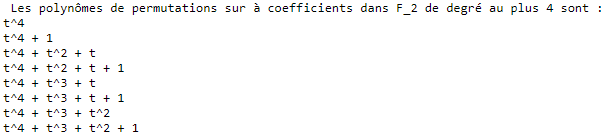
\includegraphics[width=1\textwidth]{appercu.png}
\caption{Affichage de l'exécution}
\end{figure}
\pagebreak
Nous allons ensuite présenter une implémentation sous forme algorithmique du \textbf{Critère 1} présenté précédemment. Cet algorithme est développé en \textit{Sage}.
\begin{minted}
[
frame=lines,
framesep=2mm,
baselinestretch=1,
bgcolor=LightGray,
fontsize=\footnotesize,
linenos
]
{python}
def estDePermutation(f, q):
    R.<x> = GF(q) # Corps fini à q éléments
    S.<t> = PolynomialRing(R) # Anneau de polynômes sur F_q en l'indéterminée t
    f = S(f)
    temp = t - f(R(0)) # R(0) désigne le premier élément du corps F_q
    for i in R:
        if R(0) == i:
            continue
        temp = temp * (t - f(i))
    if temp == t**q - t:
        return (True)
    return (False)
    
q = 2
deg = 4
R.<x> = GF(q)
S.<t> = PolynomialRing(R)
test1 = t**4 + t**3 + t
test2 = t**4 + t**3 + 1
answer1 = "non"
answer2 = "non"
if estDePermutation(test1, q):
    answer1 = "oui"
if estDePermutation(test2, q):
    answer1 = "oui"
print("Critère 1 :")
print("Le polynôme " + str(test1)  + " est de permutation ? " + answer1)
print("Le polynôme " + str(test2)  + " est de permutation ? " + answer2)
\end{minted}

\begin{figure}[h]
\centering
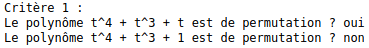
\includegraphics[width=0.68\textwidth]{appercu3.png}
\caption{Affichage de l'exécution}
\end{figure}
Cet algorithme nécessite plus de calculs que le précédent mais permet de donner une réponse directe à la question "Est ce que $P \in \mathbbm{F}_q [X]$ est de permutation ?". {\color{red} \#TODO: Donner la complexité de ces algorithmes.}
\pagebreak

Nous allons présenter aussi un algorithme permettant une implémentation du \textbf{Critère 2}. Il a été lui aussi développé en \textit{Sage}.

\begin{minted}
[
frame=lines,
framesep=2mm,
baselinestretch=1,
bgcolor=LightGray,
fontsize=\footnotesize,
linenos
]
{python}
def estDePermutation(f, q):
    R.<x> = GF(q) # Corps fini à q éléments
    S.<t> = PolynomialRing(R) # Anneau de polynômes sur F_q en l'indéterminée t
    f = S(f)
    a = t**q - t
    for element in R:
        if (a.gcd(f - element)).degree() != 1:
            return (False)
    return(True)

q = 2
R.<x> = GF(q)
S.<t> = PolynomialRing(R)
test1 = t**4 + t**3 + t**2 + 1
test2 = t**4 + t**3 + 1
answer = "non"
answer2 = "non"
if estDePermutation(test1, q):
    answer = "oui"
if estDePermutation(test2, q):
    answer2 = "oui"
print(str(test1) + " est de permutation ? " + answer)
print(str(test2) + " est de permutation ? " + answer2)
\end{minted}

\begin{figure}[h]
\centering
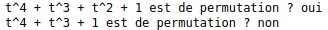
\includegraphics[width=0.5\textwidth]{appercu2.png}
\caption{Affichage de l'exécution}
\end{figure}

Cet algorithme est assez intéressant car il permet de tester directement un polynôme bien spécifique, à l'instar du premier qui permet de lister les polynômes de permutations de degré précisé.
%%%%%%%%%%%%%%%%%%%%%%%%%%%%%%%%%%%%%%%%%%%%%%%%%%%%%%%%%%%%%%%%%%%%%%%%%%%%%%%%%%%%%%%
\pagebreak

Enfin nous allons présenter une implémentation du \textbf{Critère de Hermite-Dickson}. Cette implémentation a également été réalisée en \textit{Sage}.

\begin{minted}
[
frame=lines,
framesep=2mm,
baselinestretch=1,
bgcolor=LightGray,
fontsize=\footnotesize,
linenos
]
{python}
def estDePermutation(f, q):
    R.<x> = GF(q) # Corps fini à q éléments
    S.<t> = PolynomialRing(R) # Anneau de polynômes sur F_q en l'indéterminée t
    f = S(f)
    a_pk = []
    for i in range(0, q-2):
        if p % k != 0:
            a_pk.append(i)
    for j in a_pk:
        if (f(t)**j % (t**q - t)).degree() > q - 1:
            return (False)
    if (f(t)**(q-1) % (t**q - t)).degree() == q - 1:
        return (True)
    return (False)
    
q = 2
deg = 4
R.<x> = GF(q)
S.<t> = PolynomialRing(R)
test1 = t**4 + t**3 + t
test2 = t**4 + t**3 + 1
answer1 = "non"
answer2 = "non"
if estDePermutation(test1, q):
    answer1 = "oui"
if estDePermutation(test2, q):
    answer1 = "oui"
print("Critère Hermite-Dickson :")
print("Le polynôme " + str(test1)  + " est de permutation ? " + answer1)
print("Le polynôme " + str(test2)  + " est de permutation ? " + answer2)
\end{minted}

\begin{figure}[h]
\centering
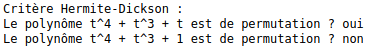
\includegraphics[width=0.5\textwidth]{appercu4.png}
\caption{Affichage de l'exécution}
\end{figure}

Cet algorithme est le plus complexe et est celui qui nécessite le plus d'opérations. Il est en revanche plus intéressant en termes de développement et de structures car il utilise des calculs plus conséquents.

\pagebreak
%%%%%%%%%%%%%%%%%%%%%%%%%%%%%%%%%%%%%%%%%%%%%%%%%%%%%%%%%%%%%%%%%%%%%%%%%%%%%%%%%%%%%%%

\section{Classes de polynômes}
Les méthodes d'identifications que nous venons de voir sont certes fonctionnelles, mais non raffinées. Elles sont extrêmement coûteuses en terme de puissance de calcul. Il est donc primordial d'établir une liste de critères permettant d'accélérer le processus. Cette partie y sera entièrement consacrée. Pour ce faire, nous travaillons sur des ''familles'' de polynômes. Nous n'aurons pas la prétention d'en donner une liste exhaustive; cependant dans ce premier rendu nous donnerons les plus élémentaires. Une étude plus approfondie sera faite au second semestre.

\subsection{Polynômes exceptionnels}
Avant de commencer, rappelons la 

\begin{prop}
L'ensemble $\Fq[X,Y]$ des polynômes en les indéterminées $X$ et $Y$ à coefficients dans $\Fq$ est muni d'une structure d'anneau, et est construit comme suit :
\begin{center} $\Fq[X,Y] = (\Fq[X])[Y] = (\Fq[Y])[X]$ \end{center}
\end{prop}

\begin{definition}
Un polynôme en les deux indéterminées $X$ et $Y$ est dit absolument irréductible s'il est irréductible sur toute extension de $\Fq$. En d'autres termes, s'il est irréductible sur la clôture algébrique $\overline{\Fq}$ de $\Fq$. 

\begin{rem}
On rappelle que toute extension de $\Fq$ est algébrique, il en va de même de sa clôture.
\end{rem}

\end{definition}
On se donne une suite d'entiers $(m_i)_{i \geq 1}$ avec $m_i \geq 1$ qui tend vers $+ \infty$. On la construit en outre de telle sorte que $\forall i \geq 1$, $m_i$ divise $m_{i+1}$ et $i$ divise $m_i$. Pour fixer les idées on prend $m_i = i !$. On pose $K_0 = \mathbbm{F}_p$ et pour tout $i \geq 1$, soit $K_i$ un corps de décomposition sur $K_{i-1}$ du polynôme $X^{p^{m_i}} - X$. Alors $K_i \cong \mathbbm{F}_{p^{m_i}}$ et on a une suite croissante
\begin{center}
$K_0 \subseteq K_1 \subseteq K_2 \subseteq ...$
\end{center}
\begin{definition}
On appelle clôture algébrique de $\mathbbm{F}_p$ notée $\overline{\mathbbm{F}_p}$ la réunion des $K_i$ :
\begin{center}
$\overline{\mathbbm{F}_p} = \displaystyle \bigcup_{i \geq 1} K_i$.
\end{center}
\end{definition}

\begin{definition}
On dit qu'un polynôme en l'indéterminée $X$ est exceptionnel sur $\Fq$ si aucun facteur irréductible du polynôme en les indéterminées $X$ et $Y$
\begin{center}
$\Psi (X,Y) := \displaystyle\frac{P(X) - P(Y)}{X-Y}$
\end{center}
n'est absolument irréductible. En d'autres terme, si les facteurs irréductibles admettent une décomposition sur une extension de $\Fq$.
\end{definition}

Avant de nous aventurer dans l'énoncé de critères, voyons un premier exemple de polynôme exceptionnel.

\begin{example}
Considérons le polynôme $P(X) := X^3 +3X^2 + 3X \in \Fq$, où $q$ est choisit tel qu'il soit la puissance d'un nombre premier impair. \newline
Construisons le fameux polynôme $\Psi(X,Y)$ à partir de $P$ :
	\begin{align*}
\Psi(X,Y) &= \displaystyle\frac{P(X) - P(Y)}{X-Y} \\
&= \displaystyle\frac{X^3 + 3X^2 + 3X - Y^3 - 3Y^2 - 3Y}{X -Y} \\
&= \displaystyle\frac{X^3 - Y^3 + 3X^2 - 3Y^2 + 3X - 3Y}{X -Y} \\
&= \displaystyle\frac{(X-Y)(X^2+Y^2) - XY^2 + YX^2 + 3(X+Y)(X-Y) +3X - 3Y}{X -Y} \\
&= \displaystyle\frac{(X-Y)(X^2+Y^2) + XY(X-Y) + 3(X+Y)(X-Y) +3X - 3Y}{X -Y} \\
&= \displaystyle X^2+Y^2 +XY+ 3(X+Y) +3\\
&= X^2 + (3+Y)X + Y^2 + 3Y + 3
	\end{align*}
Nous avons donc un polynôme de degré 2 en l'indéterminée $X$. Faisons une étude de discriminant. \newline
$\Delta_{\Psi(X,Y)} = (3+Y)^2 - 4(Y^2 + 3Y + 3) = -3(Y+1)^2$ \newline 
Nous pouvons dès à présent distinguer deux cas: 
	\begin{itemize}
		\item -3 est un carré dans $\Fq$, i.e. $\exists c\in \Fq$ tel que $c^2 = -3$. Les racines de $\Psi$ existent donc et 
			\begin{center} $\Psi(X,Y) = (\displaystyle X - \frac{-Y -3 + c(Y+1)}{2})( X - \frac{-Y -3 - c(Y+1)}{2})$.\end{center}
Ces facteurs étant de degré 1, il est clair qu'ils sont irréductibles sur toute extension de $\Fq$. $\Psi$ présente donc des facteurs absolument irréductibles, il n'est donc pas un polynôme exceptionnel.
		\item dans le cas contraire, $\Psi(X,Y)$ est irréductible dans $\Fq[X,Y]$. Cependant, $-3$ sera par définition un carré dans la clôture algébrique de $\Fq$ (Il suffit de considérer le polynôme $X^2 - 3$...). Nous sommes donc dans la même situation que dans le premier cas, à la subtilité près que cette fois-ci, $\Psi$ admet des facteurs irréductibles dans une extension de $\Fq$ et non dans $\Fq$. Donc, peu nous importe la réductibilité de ces dit facteurs ! Il s'ensuit que, par définition, $\Psi$ est un polynôme exceptionnel.
		\end{itemize}
\end{example}

Énonçons maintenant un critère fondamental :

\begin{crit}
Tout polynôme exceptionnel à coefficients dans $\Fq[X]$ est un polynôme de permutation.
\end{crit}

\begin{example}
De l'exemple précédent, il découle que $P := X^3 +3X^2 + 3X$ est un polynôme de permutation si $-3$ n'est pas un carré dans $\Fq$. \newline
Dans $\mathbbm{F}_5 \simeq \mathbbm{Z}/5\mathbbm{Z}$, $-3 = 2$ qui n'est pas un carré, donc $P$ est un polynôme de permutation. En revanche, dans $\mathbbm{F}_3 \simeq \mathbbm{Z}/ 3\mathbbm{Z}$, $-3 = 0 = 9 = 3^2$, donc $P$ n'est pas un polynôme de permutation.
\end{example}

\begin{rem}
La réciproque de ce théorème est fausse. Même s'il existe des conditions sous lesquelles elle a lieu, nous nous contenterons de donner un contre exemple.
\end{rem}

\begin{example}
Soit $q = p^n$ une puissance d'un nombre premier quelconque. Soit $P := X^p$, nous avons clairement $pgcd(q-1, p) = 1$. La \textit{Proposition 4} nous assure donc que $P$ est un polynôme de permutation. Calculons une nouvelle fois le fameux polynôme $\Psi(X,Y)$ à partir de $P$ :
	\begin{align*}
\Psi(X,Y) &= \displaystyle\frac{P(X) - P(Y)}{X-Y} \\
&= \displaystyle\frac{X^p - Y^p}{X-Y} \\
&= \displaystyle\frac{(X-Y)^p}{X-Y} \hspace{0,5cm} \text{(on travaille sur un corps de caracteristique $p$)} \\
&= (X-Y)^{p-1}
	\end{align*}
Or, les $(X-Y)$ sont évidemment irréductibles sur toute extension de $\Fq$, donc $P$ n'est pas un polynôme exceptionnel.
\end{example}
Nous allons maintenant énoncer une proposition, qui sera admise pour le moment. Sa démonstration s'appuie sur des éléments complexes de la théorie de \textit{Galois}. Nous nous laissons l'opportunité de le démontrer en ce second semestre.

\begin{prop}
Soit $q = p^n$ une puissance d'un nombre premier quelconque. Soit $k \in \mathds{N}$ tel que $pgcd(k, q-1) > 1$. Alors, il n'existe pas de polynôme exceptionnel à coefficients dans $\Fq$ de degré $k$.
\end{prop}


\subsection{Polynômes linéarisés}
Nous allons maintenant nous intéresser à la notion de polynômes linéarisés qui, sous certaines conditions que nous allons évoquer, donnent lieu à des polynômes de permutation.\\

%{\color{red} La notion de polynôme linéarisé n'est peut-être pas super à employer ! Il faudrait faire des recherches plus approfondies dessus mais pour l'instant je n'ai trouvé des applications qu'en trigonométrie avec la linéarisation de polynômes en cosinus et sinus par la formule d'Euler, etc}

\begin{definition}
On appelle polynômes linéarisés de $\mathbb{F}_{p^n} = \mathbb{F}_q$ les polynômes de la forme $\sum_{i=0}^{k} a_iX^{p^i} \in \mathbb{F}_{p^n}$.
\end{definition}
Ces polynômes correspondent aux applications $\mathbb{F}_q$-linéaires.\\
Beaucoup d'exemples de polynômes de permutations peuvent être générés à partir de ce type de polynômes, c'est pourquoi nous introduisons maintenant le critère suivant :\\
\begin{crit}
Un polynôme de permutation de $\mathbb{F}_q$ est de permutation sur toutes les extensions finies de $\mathbb{F}_q$ si et seulement s'il est de la forme $ax^{p^h} + b$ avec $a \neq 0$ et $h \geq 0$.
\end{crit}

%{\color{red} Je ne trouve pas le théorème suivant très pertinent}

%\begin{theorem}
%Si $f\in \mathbb{F}_q[x]$ n'est pas de la forme $ax^{p^h} + b$, il existe une infinité d'extensions finies $\mathbb{F}_{q^r}$ de $\mathbb{F}_q$ telles que $f$ ne soient pas un polynôme de permutation de $\mathbb{F}_{q^r}$.
%\end{theorem}
Avec ce critère peuvent venir quelques théorèmes permettant d'identifier des polynômes de permutations, tels que :
\begin{prop}
Un polynôme linéarisé est de permutation si et seulement si $0$ est son unique racine dans $\mathbb{F}_{p^n}$.
\end{prop}
\begin{theorem}[Admis]
Pour tout polynôme linéarisé $L \in \mathbb{F}_q[x]$, il existe $a \in \mathbb{F}_q$ tel que $L(x) - ax$ soit un polynôme de permutation.
\end{theorem}

Pour montrer que ces polynômes sont de permutation, il suffit bien évidemment de montrer leur bijectivité, ce qui se fait assez aisément.


%%%%%%%%%%%%%%%%%%%%%%%%%%%%%%%%%%%%%%%%%%%%%%%%%%%%%%%%%%%%%%%%%%%%%%%%%%%%%%%%%%%%%%%
\pagebreak
%%%%%%%%%%%%%%%%%%%%%%%%%%%%%%%%%%%%%%%%%%%%%%%%%%%%%%%%%%%%%%%%%%%%%%%%%%%%%%%%%%%%%%%

\section*{Conclusion}
\addcontentsline{toc}{part}{Conclusion}

Les rappels sur les corps finis étaient primordiaux . Il était nécessaire de bien définir l'environnement sur lequel nous allions travailler, d’être pourvu de bases solides, de manière à énoncer limpidement les premières définitions et propriétés des polynômes de permutations sur les corps finis. L'étude de ces polynômes est un vaste domaine des mathématiques. Il trouve de nombreuses applications, notamment en cryptologie. Nous avons ici tâché de nous en tenir aux points essentiels de leur étude, de manière à ne pas saturer notre travail d’informations superflues. \newline
\break
Il est fréquent qu'un polynôme de permutation présentant une apparence complexe, ne correspond finalement qu’à une permutation simple. Et réciproquement, une permutation compliquée sera généralement « représentable » par un polynôme de permutation simple. En tant qu’étudiant en cryptologie, cela ne peut que nous ravir. L’implémentation en sera d’autant plus facile, et ainsi l’application en cryptologie. \newline
Ceci nous a conduit, tout du long, à exhiber différents critères d’identifications et à implémenter certains d’entre eux. Ces derniers permettent de décider quels polynômes sont, ou non, de permutations ; et donc à fortiori d'en trouver de « bons » pour une application en cryptologie. \newline
Notre principale préoccupation est de trouver des algorithmes déterministes efficaces.  C’est à dire effectuant les calculs souhaités en un temps au plus polynomial. Notons toutefois que les algorithmes actuels commencent à donner des résultats en temps satisfaisant.\\
{\color{red} Guys, il faudrait présenter des algorithmes probabilistes aussi, non ? Mais S2 j'imagine ?
Répondez directement en-dessous de ce message}

%%%%%%%%%%%%%%%%%%%%%%%%%%%%%%%%%%%%%%%%%%%%%%%%%%%%%%%%%%%%%%%%%%%%%%%%%%%%%%%%%%%%%%%
\pagebreak
%%%%%%%%%%%%%%%%%%%%%%%%%%%%%%%%%%%%%%%%%%%%%%%%%%%%%%%%%%%%%%%%%%%%%%%%%%%%%%%%%%%%%%%


\section*{Références}
\addcontentsline{toc}{part}{Références}

\end{document}
